The typographic correction module receives the message with the structure given by the preprocessing module and detects the typographic errors present in the given e-mail. As it is shown in Figure \ref{fig:umltypo}, this UML package has four different UML classes: \textit{TypoCorrectorApp}, \textit{TypoCorrector}, \textit{CorrectedMessage} and \textit{Correction}.

\begin{figure}[p]
	\centering%
	\centerline{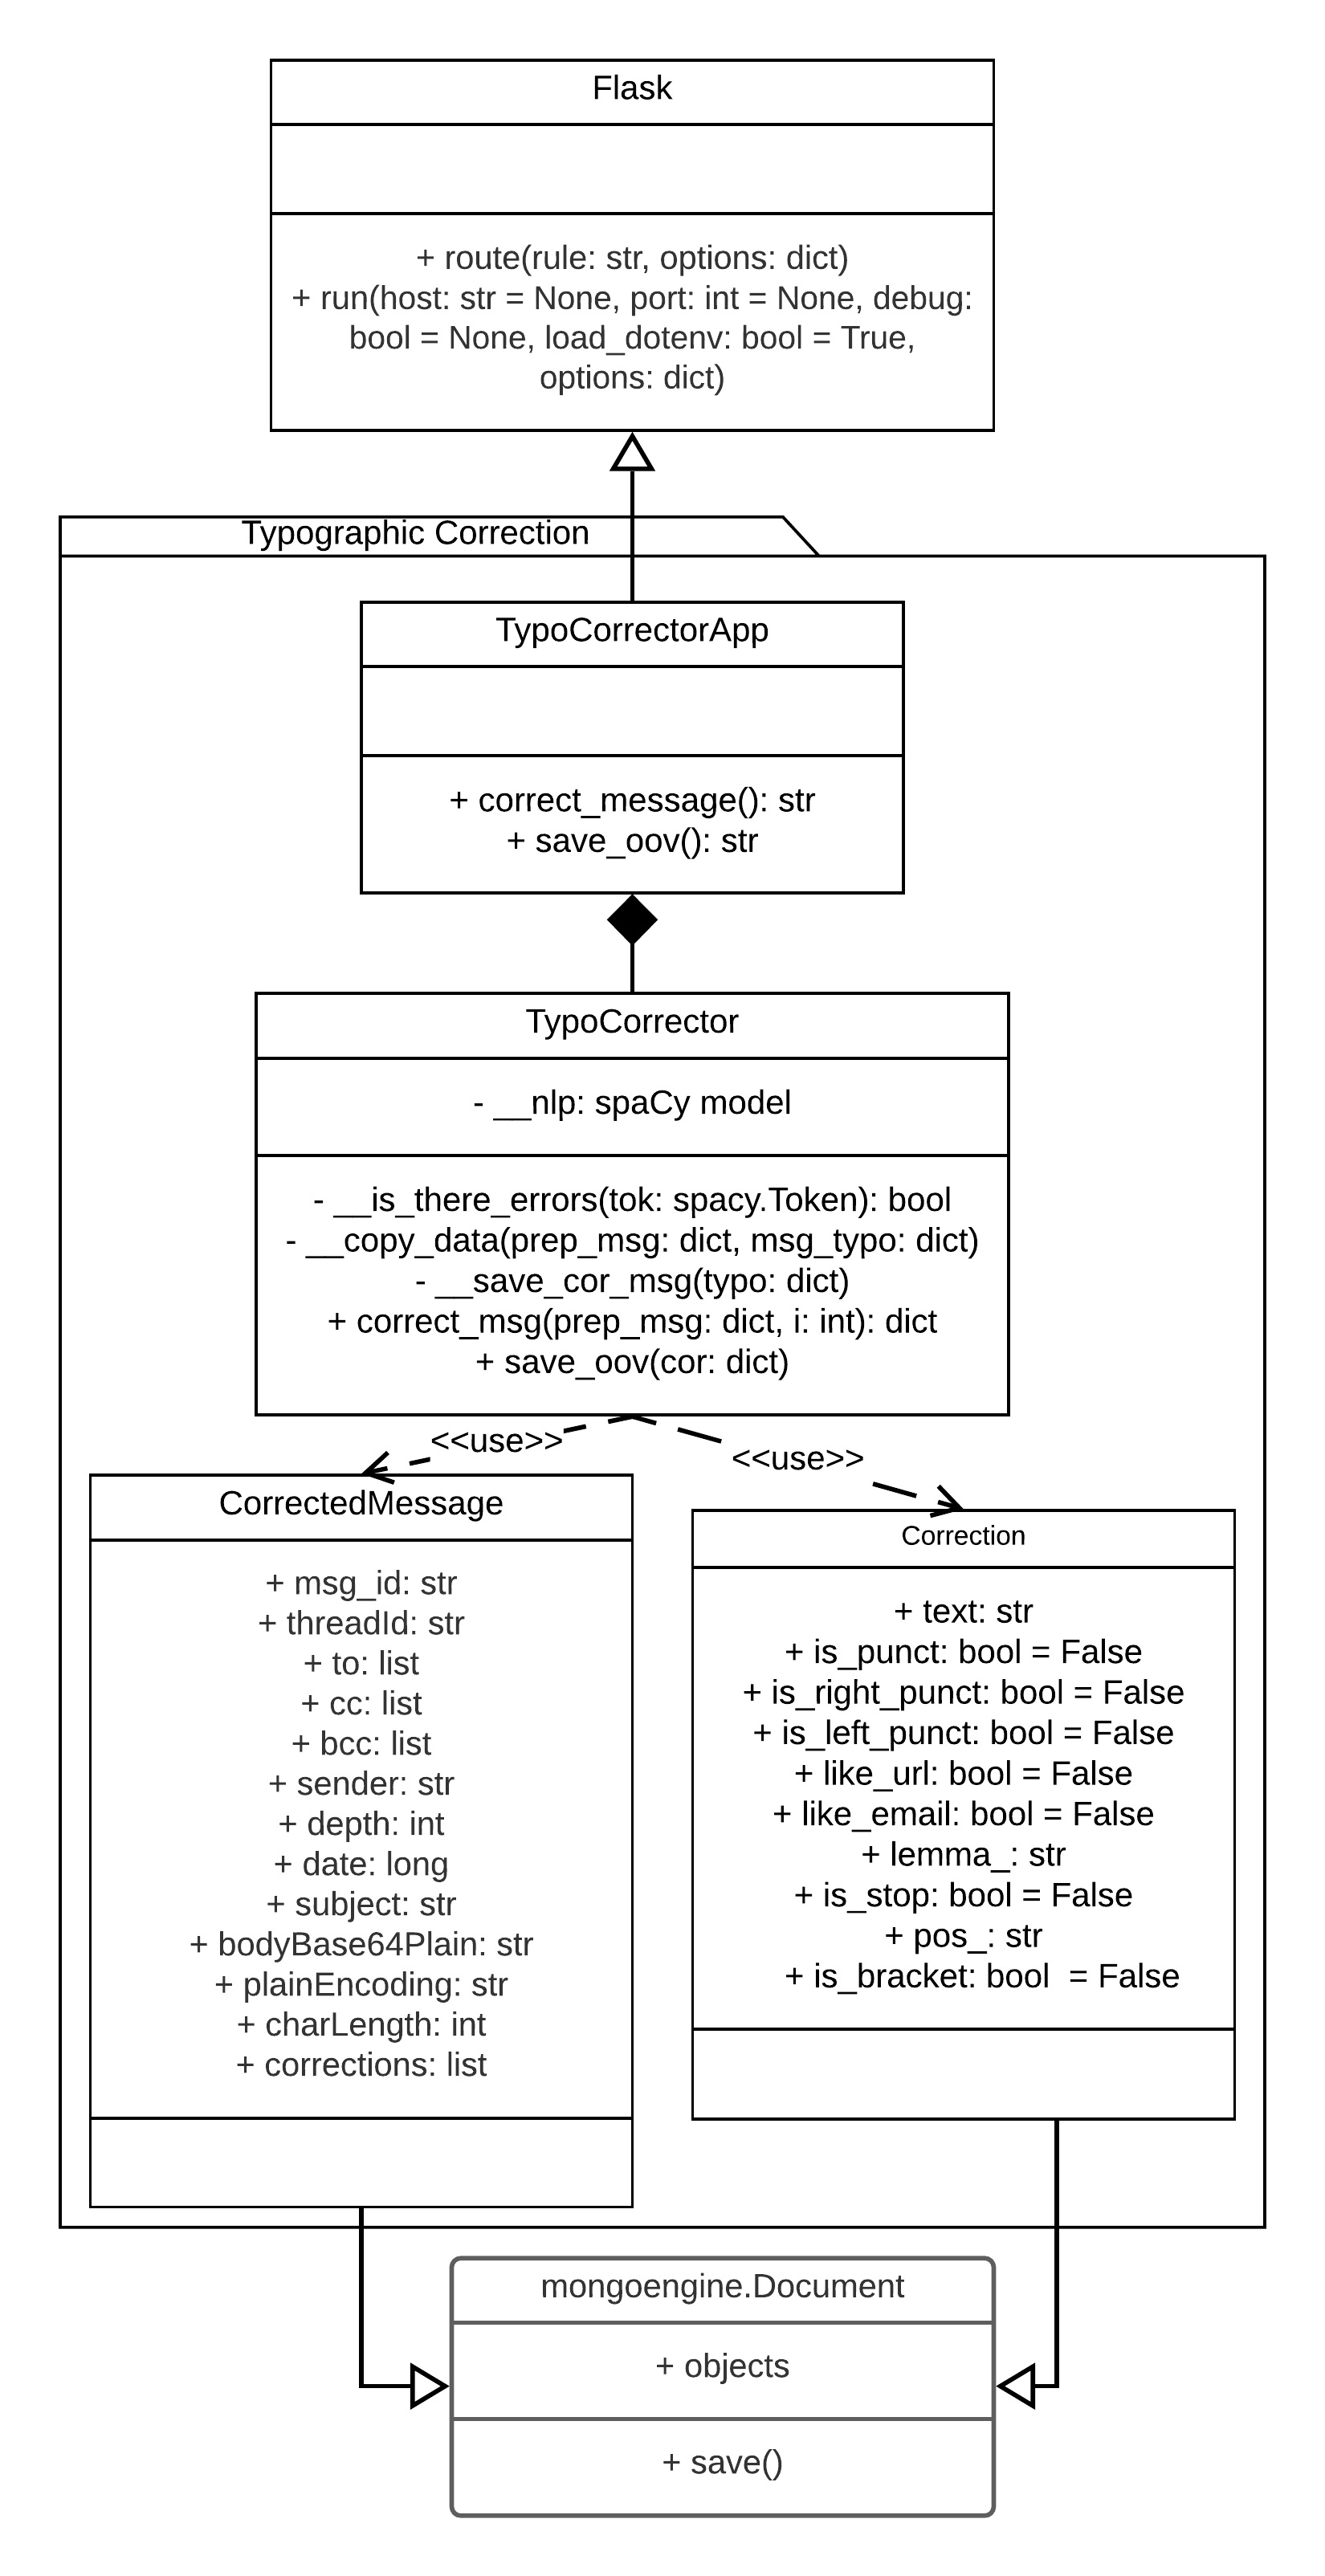
\includegraphics[width=0.9\paperwidth]{Imagenes/Bitmap/Analyser/typoUML.png}}%
	\caption{UML class diagram of the typographic correction module}%
	\label{fig:umltypo}
\end{figure}

As it happened with \textit{PreprocessorApp}, \textit{TypoCorrector} inherits from \textit{Flask} class and, thanks to it, this class implements a simple web service. However, unlike \textit{PreprocessorApp}, \textit{TypoCorrector} has two different methods which carry out different tasks. These two functions correspond to the two \textit{TypoCorrector}'s public method with the same name. Thus, if we want to invoke one of these public methods, it will be necessary to execute a POST HTTP request with an e-mail, in order to be corrected (in the case of the method \textit{correct\_msg}), or with the unrecognised token (which has been wrongly classified as ``out of vocabulary'' by our spaCy's model) that is going to be saved (we will explained both tasks in detail later). Each one of them is going to have a different url address.

The main class of this UML package, as it happens with the rest of packages, is the \textit{TypoCorrector} class. It is in charge of detecting the typographic errors and correcting them if it is possible. For this purpose it makes use (as an attribute) of an spaCy's pretrained model, specifically the one called \textit{es\_core\_news\_md}\footnote{\url{https://spacy.io/models/es}}.

The first public method that we are going to explain is \textit{correct\_msg}, which receives as parameters a message and an index. The method's parameters are originally a preprocessed message with its structure and the index as 0, which indicates that the e-mail must be corrected from the beginning, because it points the word from which the typographic correction should be made. When the function finishes its operations, it returns a dictionary with the following structure:

\begin{python}
{
	'typoCode': <enum 'TypoCode'>,
	'index': int,
	'typoError': str,
	'token_idx': int,
	'message': {
		'id' : string,
		'threadId' : string,
		'to' : [ string ],
		'cc' : [ string ],
		'bcc' : [ string ],
		'sender' : string,
		'depth' : int,               # How many messages precede it
		'date' : long,               # Epoch ms
		'subject' : string,
		'bodyPlain' : string,
		'bodyBase64Plain' : string,
		'plainEncoding' : string,
		'charLength' : int,
		'corrections' : [
		{
			'text': str,
			'is_punct': bool,
			'is_right_punct': bool,
			'is_left_punct': bool,
			'like_url': bool,
			'like_email': bool,
			'lemma_': str,
			'is_stop': bool,
			'pos_': str,
			'is_bracket': bool,
			'position': int
		}
		]
	}
}
\end{python}

If no typographic errors are detected in the text or the user's help is not needed, the \textit{message} field is previously saved in the database, by using the \textit{CorrectedMessage} class (its attributes perfectly match with the fields of the \textit{message} field dictionary), the \textit{typoCode} field will take the value \textit{successful} and the \textit{typoError} and \textit{token\_idx} fields will take the value \textit{None}. However, in other case, the execution of the system changes.

The first task the \textit{correct\_msg} method performs is to filter those e-mails whose message body as plain text is empty, due to the preprocess could produce this result, such as in forwarded messages without new text. In this case, the \textit{typoCode} will take the value \textit{notAnalysed}.

Then, it checks from the given index onwards if one token is recognised by our spaCy's model as ``out of vocabulary''. If this happens, the word is searched in the database of corrections (which is easy to manage thanks to the \textit{Correction} class) in case it was previously stored in it as a non-out-of-vocabulary token (in this database we have all words that are not really a typographic error, but they are not recognised by our natural language processing model). If the word appears in it, the information of this ``correction'' is appended to the \textit{``corrections''} list (each of its elements has the same field as the \textit{Correction} class' attributes) and the execution continues as usual, as if no error has been detected.

On the other hand, if the detected ``out of vocabulary'' token is not in our \textit{Correction} database, which means that it could be a real typographic error or a existent word which is not recognised by our spaCy's model and not previously stored, the \textit{Analyser} class (out of this module), with the help of the user, will be in charge of determining if it is a real typographic error and correcting it in that case. For this reason, the \textit{TypoCorrect} will return the mentioned structured with the \textit{typoCode} field taking the value \textit{typoFound}, the \textit{word} one with the text of the detected token and the \textit{token\_idx} with the character position of the beginning of the found word. The \textit{index} field will always take the value of the position of the last analysed word, if there are no errors detected it will be the number of words in the message.

Once the \textit{Analyser} has determined if the given word is a real typographic error, and corrected it in that case, it will invoke again the \textit{correct\_msg} method, through a POST HTTP request, and it will send as a parameter the returned \textit{message} field (probably with the message body changed or with a new element in \textit{corrections} list) and with the corresponding index. For example, if the detected token was not a real typographic error, the index will be the position after the word (due to the previous words has been analysed yet). This is the advantage of this function, it allows us to start a new typographic correction or continue a previously started one, because it admits as the \textit{prep\_msg} parameter a preprocessed message or a partially corrected message.

In this section, we have explained when the \textit{Correction} queries are carried out, but we have not said anything about when its elements are inserted. For this purpose, the \textit{save\_oov} method was implemented. If the \textit{Analyser} determines that the returned word is not a typographic error, it can carry out a POST HTTP request in order to save the information of this word in the database for future cases.